% Chapter X

\chapter{DSMC WITH SPIN - EHRENFEST} % Chapter title
\label{ch:dsmcehr} % For referencing the chapter elsewhere, use \autoref{ch:dsmcehr}

%----------------------------------------------------------------------------------------

\begin{flushright}{\slshape    
You know more than you think you know, \\ 
just as you know less than you want to know.} \\ \medskip
--- Oscar Wilde
\end{flushright}

\bigskip

%----------------------------------------------------------------------------------------
I want to motivate/connect with previous chapter and stern gerlach. Talk about other simulation methods of the stern gerlach problem, why we have chosen not to include them and why we have decided to go with dsmc.\\
%----------------------------------------------------------------------------------------

One approach to including the effects of Majorana spin flips in our DSMC simulations would be to develop a semiclassical method \ie simulate the positions of the atoms classically using the DSMC method and simulate the internal state of the atom with a quantum mechanical approach.
One such approach might be to use the Ehrenfest theorem \cite{Ehrenfest1927} to calculate the average force applied to an atom based on its current internal state (I have given a brief pseudo-code in \autoref{lst:Ehrenfest}).
Using this method we would evolve the internal state of the atom using the Schr\"odinger equation then, using the internal state of the atom, we can calculate the expectation value of the force to use in evolving the position of the atom.\\

Unfortunately this technique is not a viable solution, as we will demonstrate in this chapter.
While we are able to capture some of the interesting physics (usually short term) of the Majorana spin flip using the Ehrenfest approach, the method fails over long simulation periods.


%----------------------------------------------------------------------------------------

\section{Simulating Schr\"odinger Equation}

To apply any sort of semi-classical approach we need to be able to accurately solve the Sch\"odinger equation.
The simplest approach would be to apply a differencing scheme directly, however the schemes that have the simplest implementation generally lack the numerical properties we require; high order accuracy, stability and conservation \cite{mi_eng}. %unitary evolution conserves probability, inherently stable. % for majorana equation can get explicit expression for u % approximation to integral equation bounded hence stable and easier for higher accuracy.

The approach we have employed here, and in \autoref{ch:dsmcmcwf}, is to make use of the unitary time evolution operator \cite{?}.
The main benefit of this approach is, as the name suggests, the operator is unitary and hence inherently conserves probability.
The unitary time evolution operator is defined as follows
\begin{equation}
    \widehat{U}(t_0,t_0+\Delta t) = \exp\left[-\frac{\imath}{\hbar}\int_{t_0}^{t_0+\Delta t} \widehat{H}(t)\,dt \right]. \label{eq:timeEvolution}
\end{equation}
That is for a time dependant Hamiltonian we can evolve the state of our wavefunction, $\vert \psi \rangle$, through a moment of time $\Delta t$, with the application of the time evolution operator\footnote{It should be made obvious here that as written in \autoref{eq:timeEvolution} the evolution is exact. We can evolve through any size time step, $\Delta t$, and obtain an exact answer.}, $\widehat{U}$,
\begin{equation*}
    \ket{ \psi (t_0+\Delta t) } = \widehat{U}(t_0,t_0+\Delta t) \ket{ \psi (t_0) }.
\end{equation*}
This method is especially useful for our two level system.
Owing to the lack of a kinetic energy term in the Hamiltonian, we can explicitly derive an expression for the $2\times2$ matrix form of $\widehat{U}$ for the immediate application to an explicit numerical scheme.
Recall from \autoref{sec:intromag} that the Hamiltonian for a magnetic moment in a magnetic field is given by
\begin{equation*}
    \widehat{H} = -\hat{\boldsymbol{\mu}} \cdot \mathbf{B},
\end{equation*}
which can be expressed in matrix form as
\begin{equation*}
    \widehat{H} = \hbar\gamma \begin{bmatrix} B_z & B_x - \imath B_y \\
                                                      B_x + \imath B_y & -B_z \end{bmatrix}.                                         
\end{equation*}
In general the magnetic field components are functions of position, which, for the atoms is a function of time.
For a general magnetic field we do not know explicitly what the time dependance will be thus we will be unable to explicitly integrate the Hamiltonian as required by \autoref{eq:timeEvolution}.
\marginpar{The integration scheme we have used here is equivalent to a left handed rectangle rule, which is of order ${\cal O}(\Delta t ^2)$. It is possible to employ higher order numerical integration methods \ie midpoint, trapezoidal, Simpson's rule, although they were found not to increase performance substantially \cite{miThesis}.}
We will instead make the assumption that our time steps are very small, $\Delta t \ll 1$, so that over the time step the Hamiltonian remains relatively constant.
In this limit we have, $\int\widehat{H}(t)\,dt = \widehat{H}(t_0)\Delta t$, so that the time evolution operator becomes
\begin{align}
    \widehat{U}(t_0,t_0+\Delta t) &= \exp\left[  -\imath\frac{g_s\mu_B\Delta t}{2 \hbar} \begin{bmatrix} B_z & B_x - \imath B_y \\
                                                      B_x + \imath B_y & -B_z \end{bmatrix} \right],\\
                &= \begin{bmatrix} \cos\theta - \imath n_z \sin\theta & -\left(n_y+\imath n_x\right)\sin\theta \\
                                   \left(n_y-\imath n_x\right)\sin\theta & \cos\theta + \imath n_z \sin\theta\end{bmatrix}, 
\end{align}
where $\theta = g_s \mu_B \Delta t \vert \mathbf{B} \vert / 2\hbar$ and $n_k = B_k / \vert \mathbf{B} \vert$ are the directional components of the magnetic field normal vector.
This simple closed form expression makes it very easy to implement the unitary evolution operator method numerically.

%------------------------------------------------

\section{Schr\"odinger Simulations}

To illustrate the efficacy of this technique we will numerically solve the original Majorana problem \autoref{eq:Majprob}.
The outcome of a spin half Majorana system is necessarily binary.
To this end in \autoref{fig:majprob} I have simulated two scenarios: a spin flip (\autoref{fig:labframeFlip}, \autoref{fig:rotframeFlip}) and a not flip (\autoref{fig:labframeNoFlip}, \autoref{fig:rotframeNoFlip}).
Each scenario is plotted in two separate reference frames: the laboratory frame and the co-rotating frame.
The laboratory frame is the frame in which the spin up direction is aligned with the $z$-axis, the co-rotating frame is the frame in which the spin up direction is aligned with the local magnetic field.
The laboratory frame is the frame in which the differential equation is set, however in this frame it can become a little confusing about whether a particular spin state is flipped our not.

In both of the simulations the direction of the magnetic field changes at $t=0$, so the orientation of the spin up direction in the lab frame also changes.
In the co-rotating frame it is always clear which state is the spin up state.

The formalism of moving between frames is actually very straight forward.
First let's calculate exactly the vectors we are talking about when we say locally aligned with the magnetic field.
These are simply \textcolor{red}{(Is it that simple? Why is this so obvious?)} the normalised eigenvectors of the hamiltonian in \autoref{Eq:MagHam}
\begin{equation}
    \ket{\uparrow,\downarrow} = \frac{1}{\sqrt{2\pm 2n_z}} \begin{bmatrix} n_z \pm 1\\
                                                                           n_x + \imath n_y \end{bmatrix}.
\end{equation}
These eigenvectors are very useful since once we have an alternative complete basis it is very straight forward to transform from one to the other by using the rotation operator\footnote{For those of you more comfortable with linear algebra, $\widehat{R}$ can be thought of as the matrix whose columns are the eigenvectors of our new orthonormal basis set, \ie $\left[\ket{\uparrow}\, \ket{\downarrow}\right]$.} $\widehat{R}$, where $\widehat{R}_{ij} = \bra{\psi_i}\left.\phi_j\right>$ so that for our spin half system we would have
\begin{equation}
    \widehat{R} = \begin{bmatrix} \bra{\uparrow_z}\left.\uparrow\right>   & \bra{\uparrow_z}\left.\downarrow\right>\\
                              \bra{\downarrow_z}\left.\uparrow\right> & \bra{\downarrow_z}\left.\downarrow\right>
              \end{bmatrix}.
\end{equation}
To move between frames we use the mapping, $\ket{\phi} = \widehat{R}^{\dagger} \ket{\psi}$.
We can also transform our differential equation such that $\partial_t \ket{\phi} = \widehat{H}' \ket{\phi}$, where $\widehat{H}'\,=\,\widehat{R}^{\dagger} \widehat{H} \widehat{R}$.
I would like to comment on the form of the transformed equation, but I cannot get it into a simplified form at the moment. I should check out my honours thesis or talk to Russ, it is all in there, although it has been framed with a different language.

\begin{figure}
\hspace{-6em}
\makebox[1.8\linewidth][l]{%
\centering
\subfloat[Lab frame flip, $B_t=1\times10^{-7}$]{\label{fig:labframeFlip}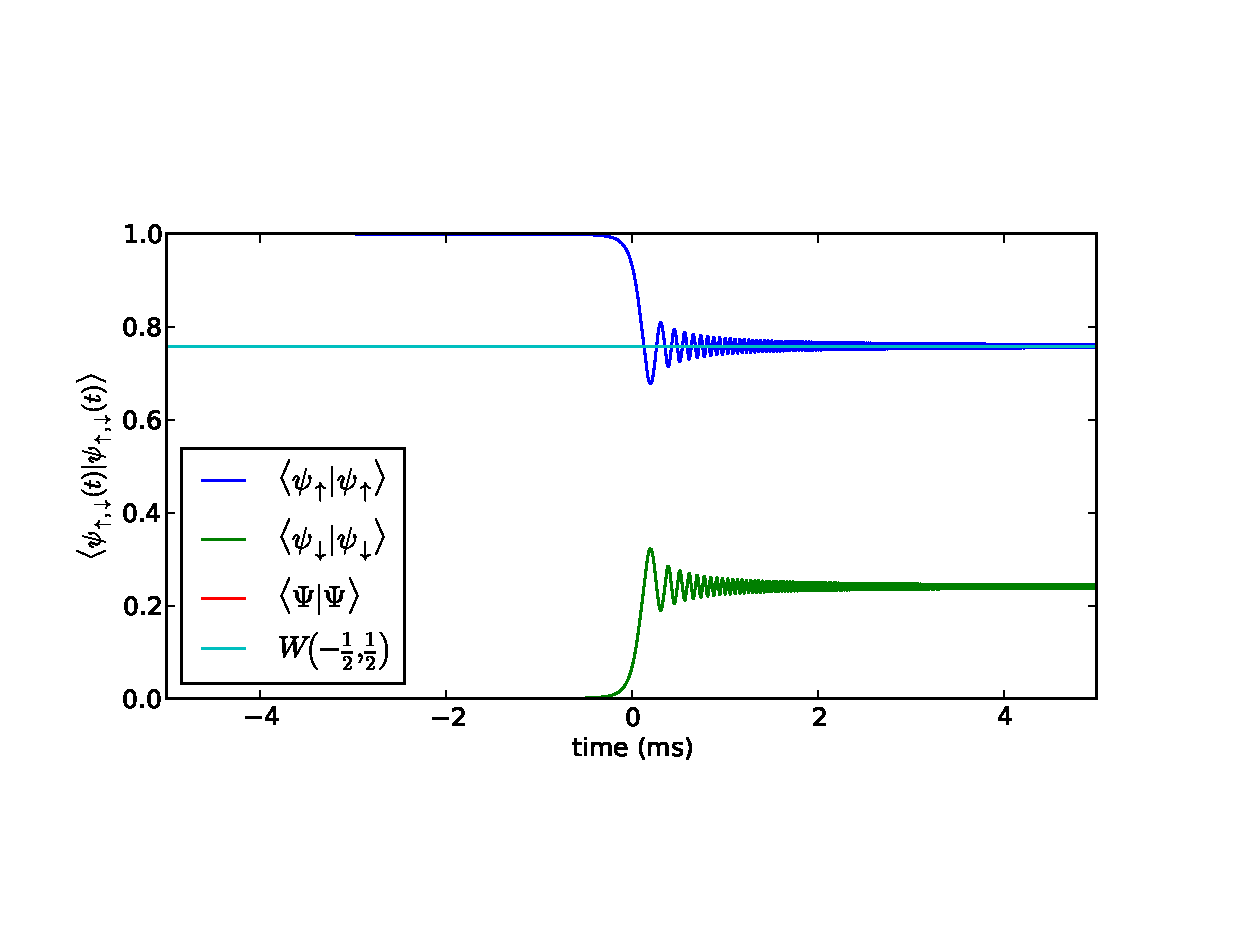
\includegraphics[width=0.75\textwidth]{gfx/Ehrenfest/labframeFlip}}\quad
\subfloat[Rotating frame flip]{\label{fig:rotframeFlip}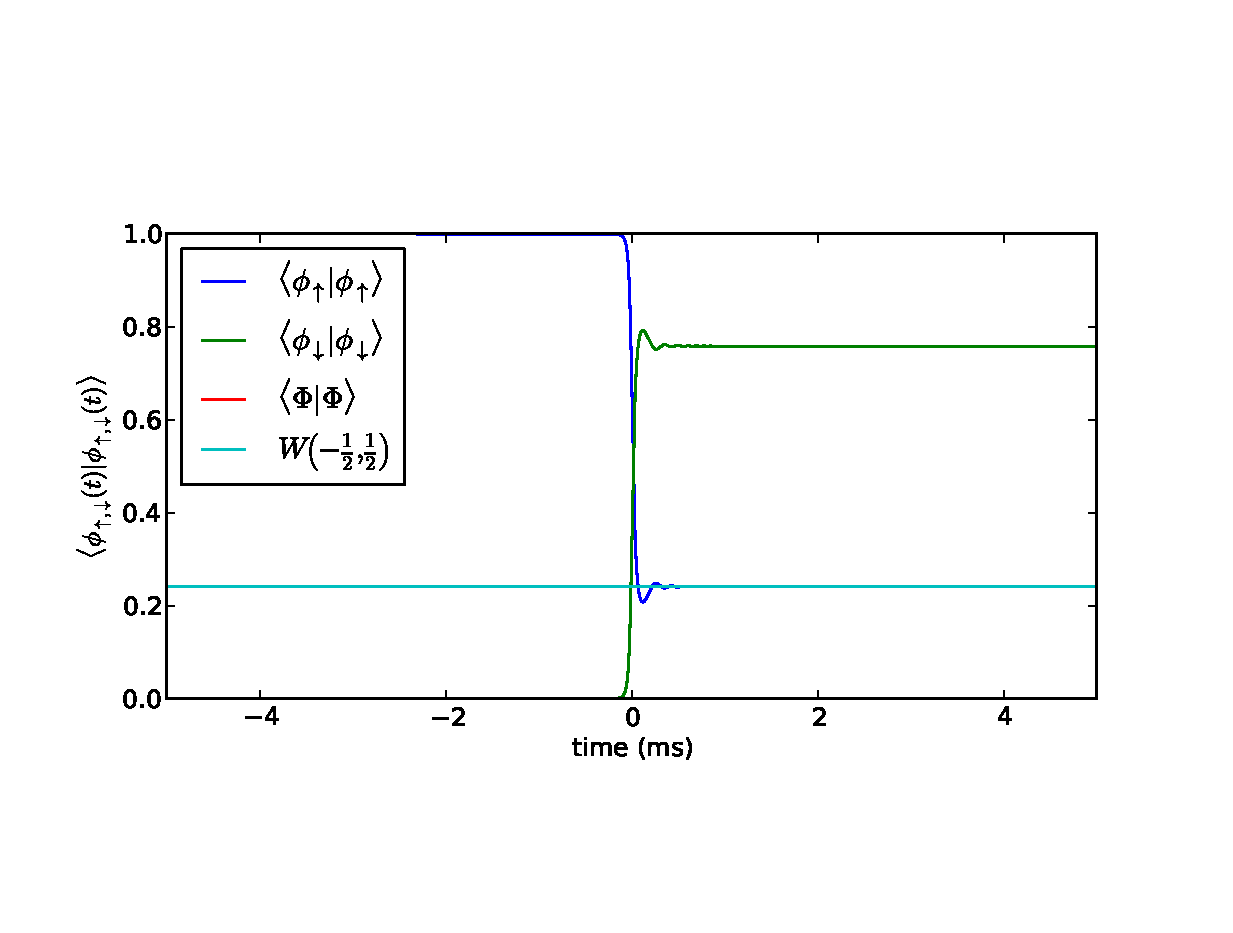
\includegraphics[width=0.75\textwidth]{gfx/Ehrenfest/rotframeFlip}}
}\\\_
\hspace{-6em}
\makebox[1.8\linewidth][l]{%
\centering
\subfloat[Lab frame no flip, $B_t=2\times10^{-7}$]{\label{fig:labframeNoFlip}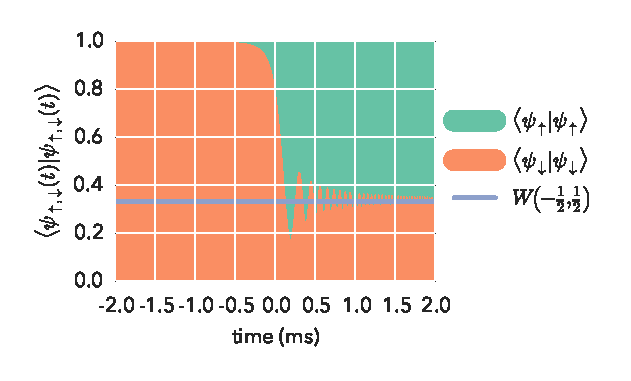
\includegraphics[width=0.75\textwidth]{gfx/Ehrenfest/labframeNoFlip}}\quad
\subfloat[Rotating frame no flip]{\label{fig:rotframeNoFlip}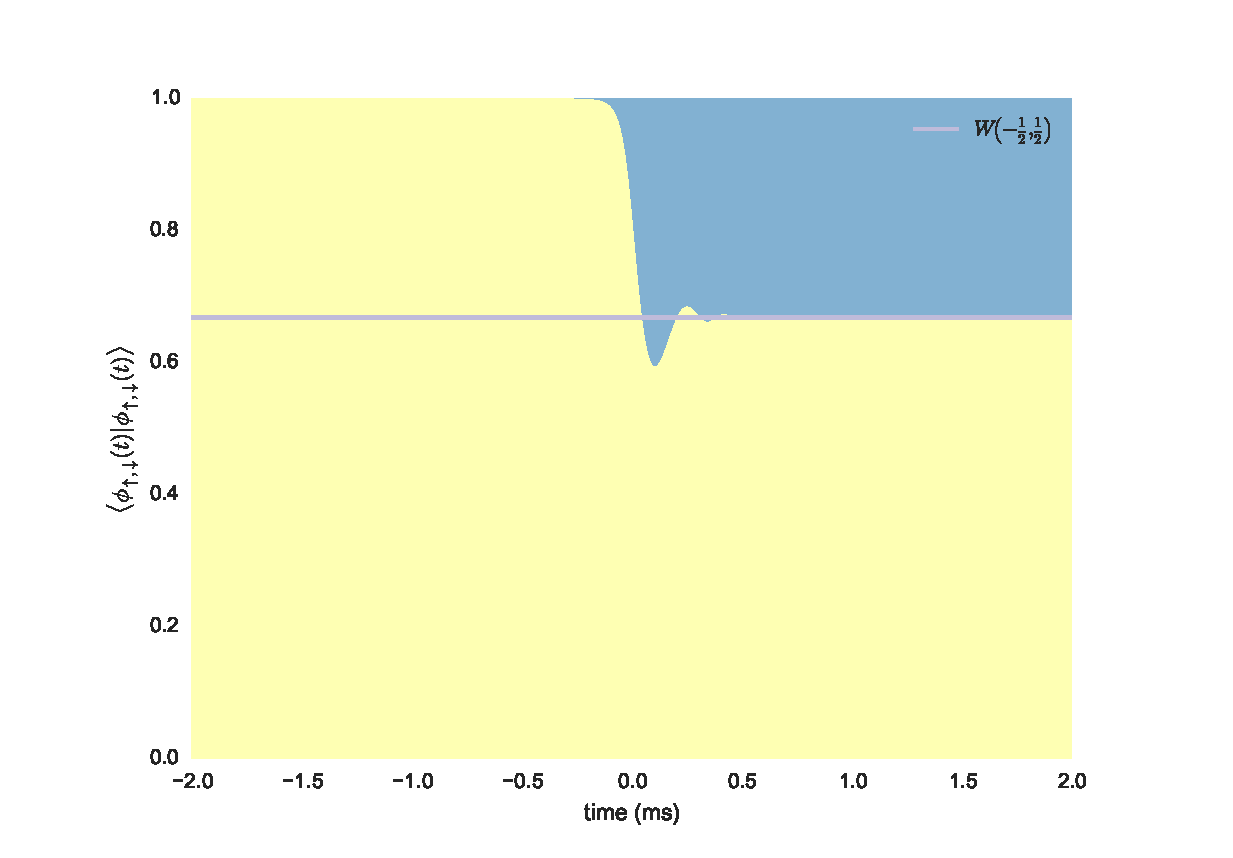
\includegraphics[width=0.75\textwidth]{gfx/Ehrenfest/rotframeNoFlip}}
}
\caption{Simulating the no majorana spin flip }\label{fig:majprob}
\end{figure}

\autoref{fig:labframeFlip} and \autoref{fig:rotframeFlip} both illustrate a Majorana spin flip.
In this simulation we used the magnetic field $\mathbf{B}=(0.1,0.0,2500t)\,\mathrm{mT}$, and began at $t=-15\,\mathrm{ms}$ where the population in the spin down component in the lab frame is less than $10^{6}$ (we have plotted a smaller time window in \autoref{fig:majprob}). \textcolor{red}{(Not sure what that sentence was supposed to be about? Maybe it is alking about the number of simulated atoms?)}
We can see the distinct different between the behaviour of the spin populations in the two different reference frames.
The initial wavefunction was chosen such that the population of the spin up component in the lab frame was 1.
\autoref{fig:rotframeFlip} clearly displays a change in the most probable state, whereas in \autoref{fig:labframeFlip} it is not so clear.
Again this is because in the lab frame the spin up direction changes at $t=0$ when the sign of the $z$ component of the magnetic field moves from negative to positive.
\autoref{fig:labframeNoFlip} and \autoref{fig:rotframeNoFlip} results from a simulation with $\mathbf{B}=(0.2,0.0,2500t)\,\mathrm{mT}$.
In these plots we see the converse behaviour in the state populations, indicating that no spin flip has occurred.

For both simulations we have used a time step of $\Delta t = 1\,\mu\mathrm{s}$.
This may seem overkill given the rate of change of the magnetic field can be characterised by $\tau_B=\vert\mathbf{B}\vert / \partial_t\vert\mathbf{B}\vert = 15\,\mathrm{ms}$ at the beginning of the simulation.
However there is another time scale that must be considered in a simulation like this, that is the period of a Larmor precession, $T_L = 2\pi\hbar / g_s \mu_B \vert\mathbf{B}\vert = 3.81\,\mu\mathrm{s}$ at the begining of the simulation.
While we do not expect the spin to precess for the first half of the simulation when it is completely aligned with the magnetic field, it is the period close to the field minimum and beyond that will experience Larmor precession.
In fact the wiggles after the spin flip occur at the Larmor precision frequency.
For example, look at one period of oscillation around $t=0.3\,\mathrm{ms}$, here the Larmor precession period will be, $T_L=0.19\,\mathrm{ms}$, exactly as simulated (**MAKE INSET IN FIGURE TO SHOW LARMOR PRECESSION RATE**).

\marginpar{The astute reader may be confused by line 4 of the pseudo-code in listing \ref{lst:Ehrenfest}.
The appearance of the $n+1^\mathrm{th}$ velocity when calculating the $n+1^\mathrm{th}$ position is not how one might implement the standard Euler integration method. 
Here we have used an implementation of the Symplectic Euler method \cite{??}, which has better energy conserving properties than the standard forward Euler.
This technique still has the same order accuracy with time, and introduces no added computational complexity, yet we gain some extra stability in the total energy of the atom.}

%------------------------------------------------

\section{Single Atom Spin Flips} \label{sec:EhrenfestSingleAtom}

Confident in our ability to accurately simulate the Schr\"odinger equation, in our regime of interest, we may begin to apply the Ehrenfest method to simulating spin flips of real atoms.
The first step is to first see wether or not we can simulate the spin flip of a single atom.
I have given a pseudo-code example for a single time step of the Ehrenfest algorithm in \autoref{lst:Ehrenfest}\footnote{Note in \autoref{lst:Ehrenfest} that we have denoted the discrete approximation to a continuous variable as, $g_n \approx g(t_n)$.}.
\begin{lstlisting}[float,caption=Psuedo-code algorithm for a single Ehrenfest method time step, mathescape,label= lst:Ehrenfest,stepnumber=1]
Calculate force using current spin state: $\mathbf{F}_n = \bra{\Psi_n}\widehat{\mathbf{F}}_n\ket{\Psi_n}$.
Evolve wavefunction using time evolution operator: $\ket{\Psi_{n+1}} = \widehat{U}_n \ket{\Psi_{n}}$.
Evolve velocity using the average force: $\mathbf{v}_{n+1} = \mathbf{v}_n + \mathbf{F}_n \Delta t / m$.
Evolve position using the new velocity: $\mathbf{x}_{n+1} = \mathbf{x}_n + \mathbf{v}_{n+1} \Delta t$.
\end{lstlisting}

\begin{figure}
\hspace{-8em}
\makebox[1.8\linewidth][l]{%
\centering
\subfloat[Co-rotating frame spins]{\label{fig:ehrenfestSpin}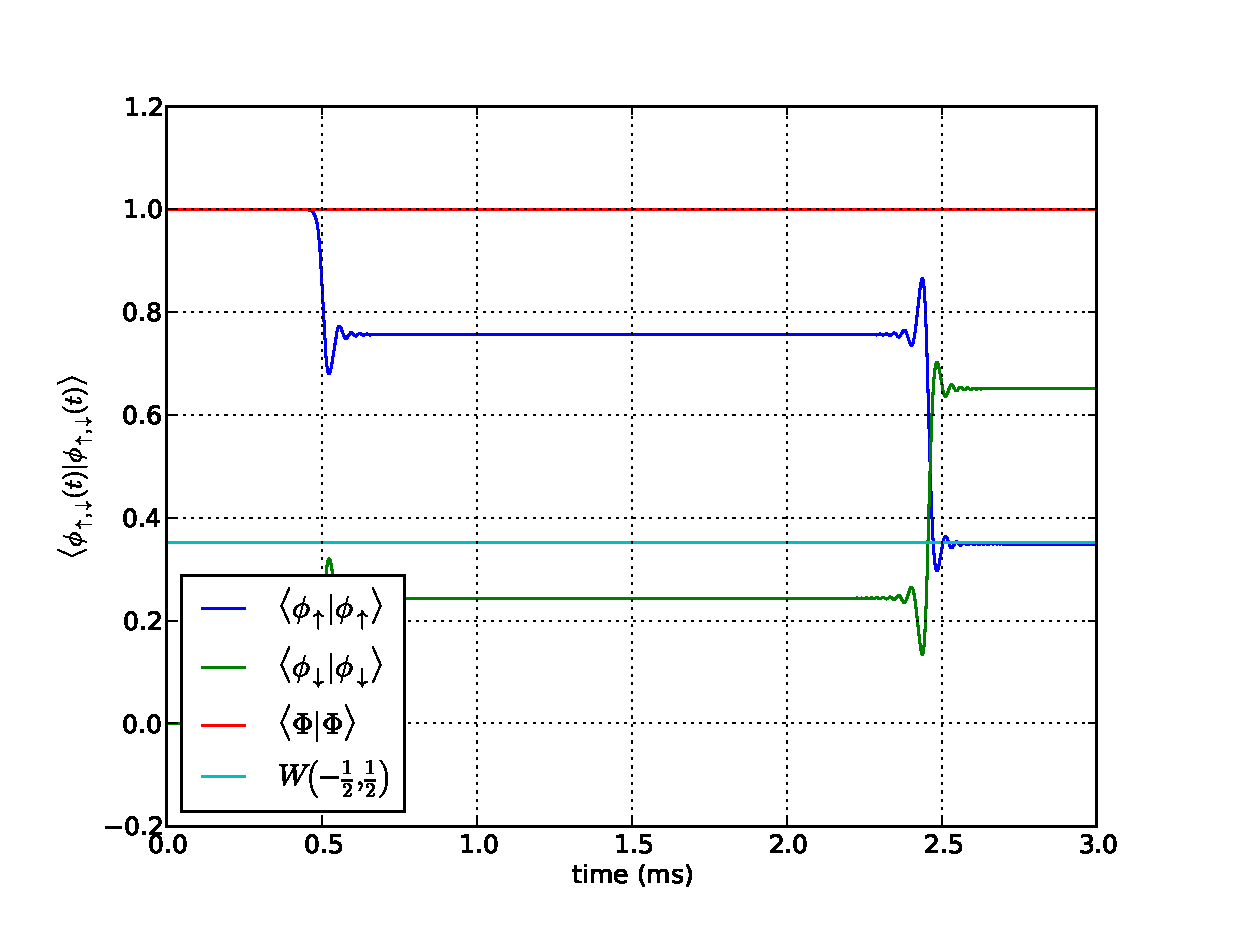
\includegraphics[width=0.525\textwidth]{gfx/Ehrenfest/ehrenfestSpin}}\quad
\subfloat[Position and velocity]{\label{fig:ehrenfestPos}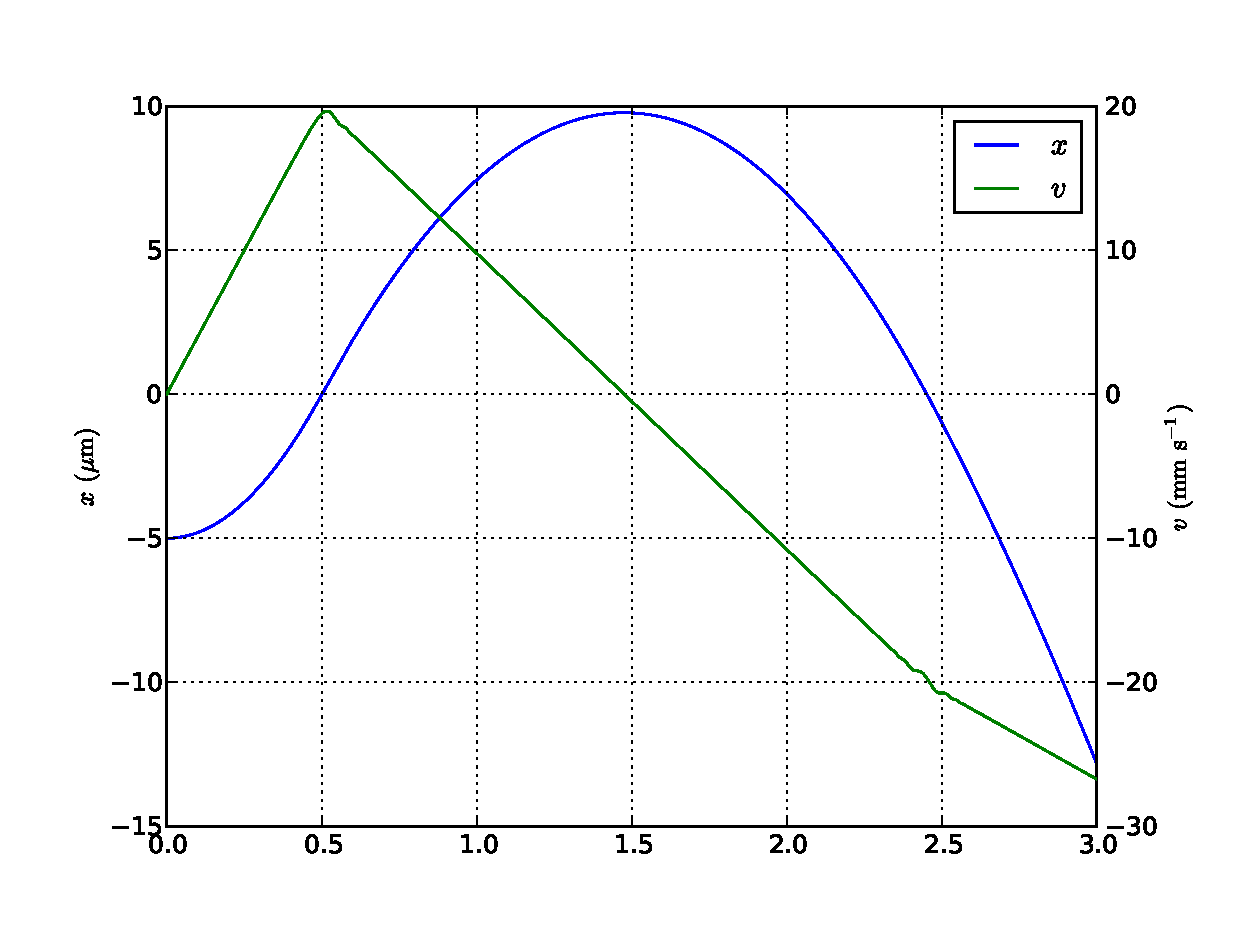
\includegraphics[width=0.525\textwidth]{gfx/Ehrenfest/ehrenfestPos}}\quad
\subfloat[Energy]{\label{fig:ehrenfestEnergy}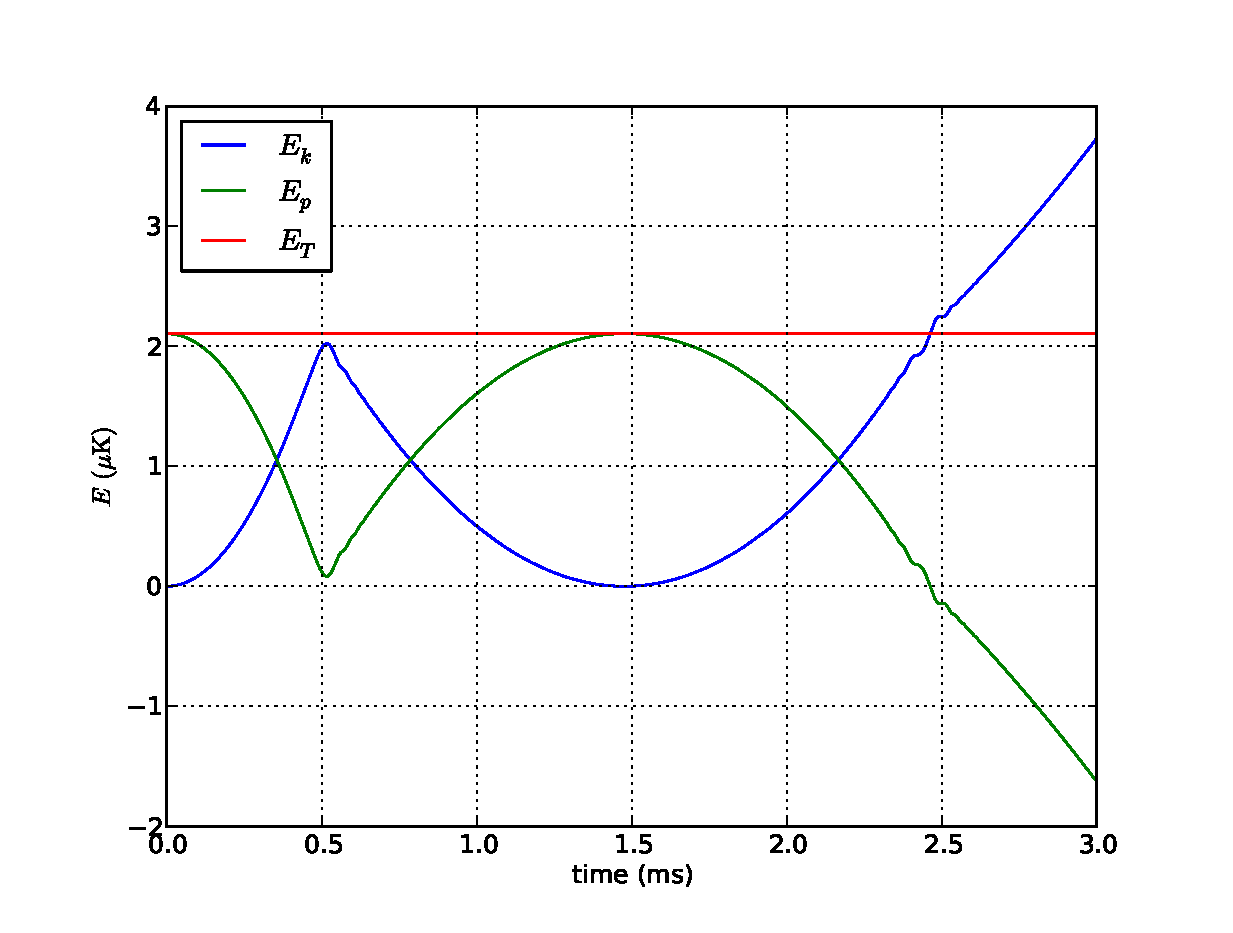
\includegraphics[width=0.525\textwidth]{gfx/Ehrenfest/ehrenfestEnergy}}%
}
\caption{No flip and flip in the same simulation.}\label{fig:ehrenfestFlip}
\end{figure}

\autoref{fig:ehrenfestFlip} shows the results from one such simulation.
This simulation was of a rubidium 87 atom that began at $z=-5\,\mu\mathrm{m}$ with a zero initial velocity.
Again the initial wavefunction was chosen so that it would be completely spin up in the co-rotating frame.
The magnetic field was given by $\mathbf{B} = (B_x,0,B_z'z)$, with $B_x=1\,\mu\mathrm{T}$ and $B_z'=2.5\,\mathrm{Tm}^{-1}$\footnote{I am aware that this magnetic field does not satisfy Maxwell's equations, but it serves as a nice example and more closely aligns with the field considered by Majorana.}.
This is a fabulous example of how well the Ehrenfest method can work.
\autoref{fig:ehrenfestSpin} displays how well the spin populations are simulated.
Again they agree with the predictions of the Majorana formula and the total probability is conserved.
\marginpar{Say how I can still use the Majorana formula here. $c =v(t=0) B_z'$.}
In \autoref{fig:ehrenfestPos} I have plotted the position and velocity of the atom as it moves through time.
We can see how the atom remains trapped after the first partial flip and is then completely ejected from the trapped once it has flipped.
Finally \autoref{fig:ehrenfestEnergy} shows how the total energy of the atom is conserved throughout the simulation (even after it has flipped).
So things seem to be working quite well, but earlier I alluded to the fact that the Ehrenfest method is not suitable to this kind of problem, so what is wrong?
I will let you stew on this few a few sections while we investigate the behaviour of a full gas simulation.

%----------------------------------------------------------------------------------------

\section{Full Gas Simulations}

Convinced that our Ehrenfest method can simulate spin flips and conserves both energy and probability we can begin to run some full gas simulations.
Majorana spin flips only occur when there is a sharp transition in magnetic field direction, like that transition that is present around the centre of a quadrupole trap.
An IP trap does not have this kind of transition, thus we would expect a very small number ($\sim 0$) of spin flips to occur as a result of the IP field configuration.
As a cautionary test we will simulate a gas trapped in an IP trap using the Ehrenfest method.

%------------------------------------------------

\subsection{Ioffe Pritchard Trap}

The IP trap will remove any of the complex dynamics (and atom loss) we would experience from Majorana loss.
This will allow us to simulate the energy and probability conserving characteristics of the method, as well as ensure that the simulated particle dynamics are as expected.

\begin{figure}
\hspace{-11em}
\makebox[1.8\linewidth][l]{%
\centering
\subfloat[IP Distribution]{\label{fig:ehrenfestIPDist}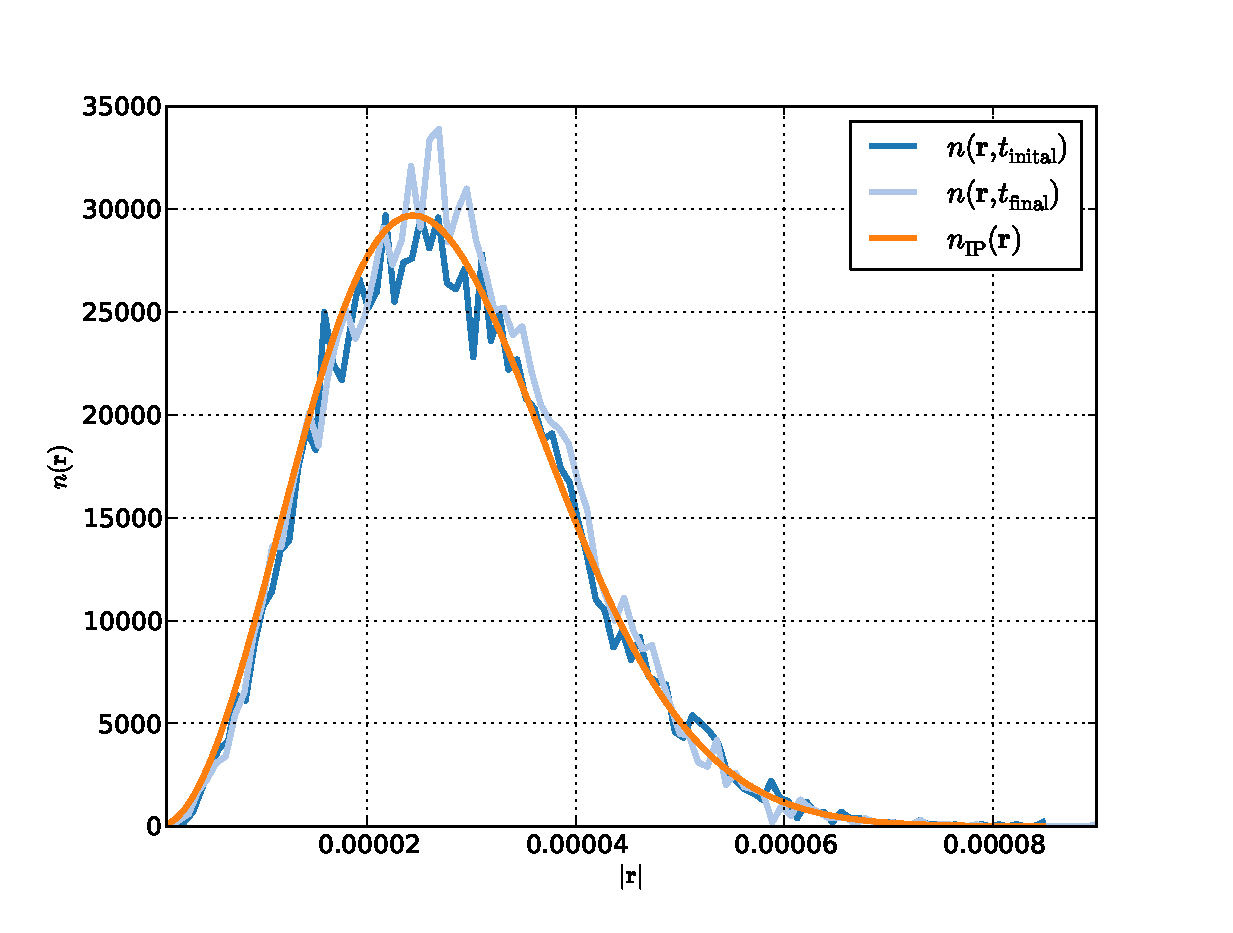
\includegraphics[width=0.75\textwidth]{gfx/Ehrenfest/ehrenfestIPDist}}\quad
\subfloat[IP Conservation]{\label{fig:ehrenfestIPCons}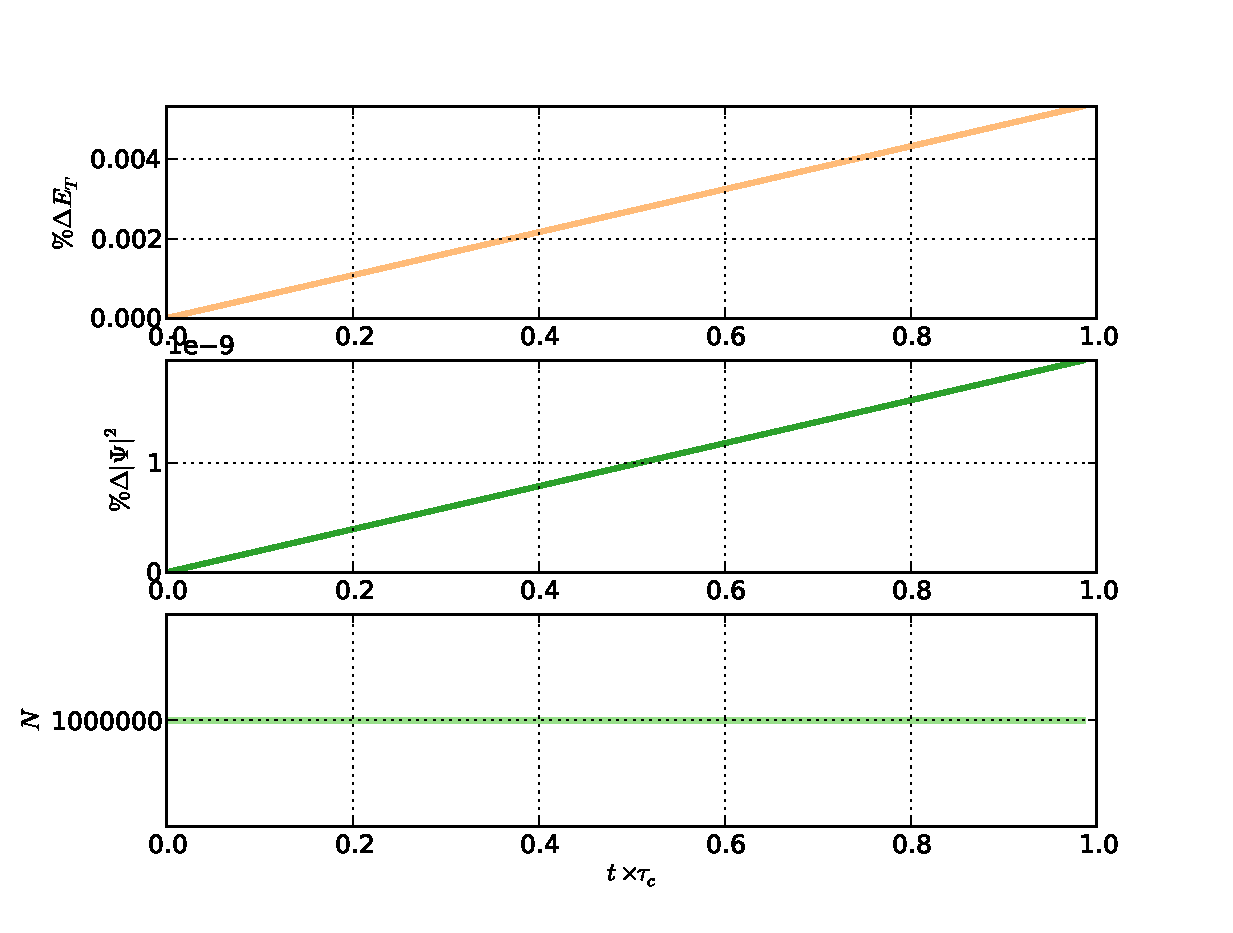
\includegraphics[width=0.75\textwidth]{gfx/Ehrenfest/ehrenfestIPConserve}}
}
\caption{Ehrenfest method for a gas in an IP trap.}\label{fig:ehrenfestIP}
\end{figure}

The results from a simulation of $10^6$ rubidium 87 atoms at $2\,\mu\mathrm{K}$ in an IP with $B_0=0.01\,\mathrm{T}$, $B'=20.0\,\mathrm{Tm}^{-1}$ and $B''=40,000\,\mathrm{Tm}^{-2}$ over a period of approximately 10 collision times ($10\tau_c$) are shown in \autoref{fig:ehrenfestIP}.
In this figure I have tried to show the conservative properties of the Ehrenfest method.
\autoref{fig:ehrenfestIPDist} illustrates the radial distribution of particles.
I have drawn the distribution at the beginning and the end of the simulation, as well as contrast it with the analytic result for a thermal gas at this temperature.
\marginpar{The density distribution for a thermal gas is $n(\mathbf{r}) = n_0 \exp\left[-\mathcal{U}(\mathbf{r})/k_BT\right]$.}
As we can see the numerical result is very stable and agrees well with the analytic prediction.
In \autoref{fig:ehrenfestIPCons} I have illustrated the change in the quantities we would expect to be conserved in a simulation like this.
The top graph shows the percentage change in the average total energy, the middle graph shows the percentage change in the average norm of the wavefunction and the bottom graph shows the number of atoms.

First of all we can note there is no change in the number of atoms \ie no Majorana spin flips.
This simulation has the same evaportaion code running as we developed in \autoref{sec:evaporation}, with the evaporation condition that if $P_z < 0$ the atom is removed.
This is due to the presence of the non-zero field bias, $B_0$, which ensures that the Larmor precession rate is always greater than the rate of change of the magnetic field direction.
Second we can see a linear increase in the total energy and wavefunction norm.
How can this be, I thought we were using fancy symplectic methods that were designed to conserve these quantities?
I have two responses to that question, the first is can we really call a \%0.005 (that is 1 in 20,000) increase a significant change?
For the simulation I have run here this corresponds to the total energy changing by $0.3\,\mathrm{nK}$, not what we might consider a significant increase in temperature.
However, we can argue that there is a clear linear trend and if we anticipate running extended simulations this might be something that we wish to keep in mind.
Although I wouldn't consider this a deal breaker.
My second response would be that the time step I have used is far too large.
For this simulation I have used the time step, $\Delta t = 5\,\mathrm{ns}$.
This might seem quite small but compared to the Larmor period at the the average radius, $T_L\approx 10^{-8}\,\mathrm{s}$, it isn't that great.
Not only does this mean on average we are only sampling the wavefunction twice per Larmor rotation, but out on the edges of the gas we are doing far worse!
Of course we could reduce the time step, and this would improve our energy conservation, but to be able to run these simulations in a reasonable time frame we must accept a certain level of non-conservation in our total energy and wavefunction norm.

Overall this seems to have worked quite well and yet I keep saying that the Ehrenfest method is not suitable for our simulations.
Let's now try to run a simulation in a quadrupole trap and see how effective the method is.
%------------------------------------------------

\subsection{Quadrupole Trap} \label{sec:EhrenfestQuad}

Content